\hypertarget{principy-hry}{%
\subsubsection{Principy hry}\label{principy-hry}}

\hypertarget{cuxedl-hry}{%
\paragraph{Cíl hry}\label{cuxedl-hry}}

Cílem je dostat obě rybičky ven. Abys toho dosáhl, musíš různě přerovnat
a přeskupit předměty v místnosti. Při tom je třeba dbát velké
opatrnosti, neboť rybičky jsou stvoření křehká a je snadno je zahubit.

\hypertarget{pravidla-pro-pohyb}{%
\paragraph{Pravidla pro pohyb}\label{pravidla-pro-pohyb}}

\hypertarget{posun-pux159edmux11btux16f}{%
\subparagraph{Posun předmětů}\label{posun-pux159edmux11btux16f}}

Jestliže rybička před sebou nějaký předmět tlačí, musí ho mít položený
na nějaké podložce.

Rybička může předmět, který se o nic neopírá, posunout jen tehdy, když
se o něco opře v nové pozici, jako třeba na obrázku vpravo.

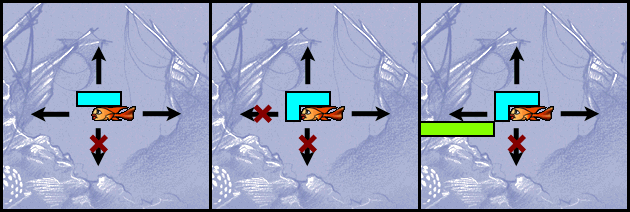
\includegraphics[width=6.5625in,height=2.20833in]{pushing_objects.png}

\hypertarget{posunovuxe1nuxed-po-jinuxfdch-pux159edmux11btech}{%
\subparagraph{Posunování po jiných
předmětech}\label{posunovuxe1nuxed-po-jinuxfdch-pux159edmux11btech}}

Není možné posunovat předmět po jiné rybičce stejně, jako rybička sama
nemůže tlačit předmět, který se o nic neopírá.

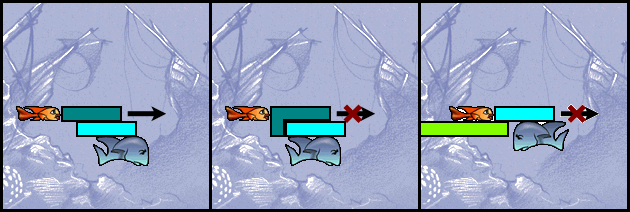
\includegraphics[width=6.5625in,height=2.20833in]{pushing_along_other_objects.png}

\hypertarget{shazovuxe1nuxed-pux159edmux11btux16f}{%
\subparagraph{Shazování
předmětů}\label{shazovuxe1nuxed-pux159edmux11btux16f}}

Padající předměty jsou vždycky smrtelné. Nezáleží na tom, co shodíte
nebo z jaké výšky; pokud předmět dopadne na rybičku nebo na něco, co se
o rybičku opírá, znamená to pro ni smrt.

Jediné případy, kdy je možné předmět po rybičce posunout, jsou situace,
kdy předmět buď hned spadne nebo se opře o podklad.

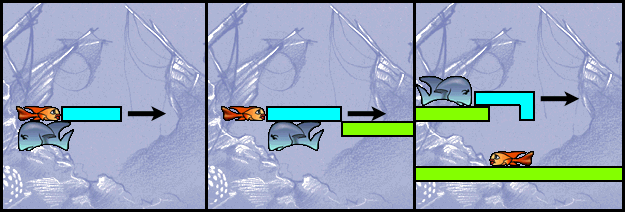
\includegraphics[width=6.51042in,height=2.20833in]{falling_objects.png}

\hypertarget{pohyb}{%
\paragraph{Pohyb}\label{pohyb}}

Svoje rybičky můžeš ovládat třemi různými způsoby:

\begin{enumerate}
\item ~
  \hypertarget{kurzorovuxfdmi-kluxe1vesami}{%
  \subparagraph{Kurzorovými
  klávesami}\label{kurzorovuxfdmi-kluxe1vesami}}

  \textbf{Klávesami nahoru, dolů, doprava a doleva ovládáš aktivní
  rybku}. \textbf{Mezerníkem se můžeš mezi rybkami přepínat}.

  Pokud se ti zdá, že ryba na tvoje pokyny nereaguje, pravděpodobně se
  snažíš odsunout něco, co není volně upevněný předmět, nebo se snažíš
  malou rybičkou posunout ocelový předmět.

  Budeš-li držet kurzorovou klávesu stisknutou, pohyb rybičky se asi po
  třech polích zrychlí.
\item ~
  \hypertarget{myux161uxed}{%
  \subparagraph{Myší}\label{myux161uxed}}

  Ukaž kurzorem myši na místo, kam chceš s rybkou dojet, stiskni a drž
  stisknuté levé tlačítko myši. Pokud tam rybka může dojet, aniž by
  něčím pohnula, vydá se na cestu. Asi po třech polích se její pohyb
  zrychlí.

  Pokud chceš nějakým předmětem pohnout, stiskni a drž stisknuté pravé
  tlačítko myši. Aktivní rybka se pohne nejkratší možnou cestou k místu,
  kam jsi ukázal.

  Mezi rybami se můžeš přepínat prostě tak, že na rybu, kterou chceš
  aktivovat, klikneš levým tlačítkem.
\item ~
  \hypertarget{pux159uxedmo}{%
  \subparagraph{Přímo}\label{pux159uxedmo}}

  \textbf{Klávesami A, S, D a W můžeš ovládat malou rybičku a klávesami
  J, K L a I velkou rybku}. Toto ovládání má jedinou výhodu - nemusíš se
  přepínat mezi rybkami.
\end{enumerate}
